The purpose of the data-preparation stage was to transform the raw Gallstone
dataset into a consistent, traceable, and modelling-ready dataset. Decisions
made during this stage were informed by the business objective, findings from
the exploratory analysis, data-quality checks, and the technical requirements
of the modelling pipeline.

All data-preparation procedures were implemented using an open-source Python
workflow. The main libraries used were \texttt{pandas} and \texttt{NumPy} for
data manipulation and validation, \texttt{SciPy} for statistical
transformations, \texttt{scikit-learn} for data partitioning and preprocessing,
and \texttt{Matplotlib} and \texttt{Seaborn} for diagnostic visualisation.

Using Python rather than a graphical modelling environment provides a
script-based and reproducible workflow in which each preprocessing operation can
be inspected, rerun, and consistently applied to subsequent modelling
experiments.


\subsection{Data Selection}
\label{subsec:data-selection}

The modelling dataset contains \textit{Gallstone Status} as the target variable
and the available demographic, comorbidity, body-composition, and laboratory
measurements as candidate predictors. Variables were initially retained rather
than removed solely on the basis of weak univariate relationships because the
exploratory analysis suggested that gallstone status may depend on combinations
of multiple patient characteristics.

Data selection was performed programmatically using Python. The dataset was
loaded into a \texttt{pandas DataFrame}, after which column names, data types,
unique values, distributions, and summary statistics were inspected. Candidate
predictors were retained when they had plausible clinical relevance and
sufficient data quality for subsequent modelling.

Variables containing unusual values, strong skewness, or high correlations with
other predictors were not immediately removed. Instead, these characteristics
were investigated during exploratory analysis and preprocessing. In particular,
highly correlated predictors were reviewed during feature selection because
multicollinearity may influence coefficient stability in models such as
logistic regression.

No patient-identifying information or variables without potential predictive
value were required for model development. Identifier fields used for data
traceability were retained during data processing but excluded from the feature
matrix supplied to the predictive models.


\subsection{Data Cleaning}
\label{subsec:data-cleaning}

Data cleaning was guided by the issues identified during the earlier
data-quality assessment. The Python workflow systematically evaluated missing
values, duplicated records, invalid categorical codes, numerical ranges, data
types, and potential extreme observations.

Completeness was assessed using functions such as
\texttt{DataFrame.isna()}, while duplicate observations and field-level
consistency were examined using standard \texttt{pandas} operations. Summary
statistics and value-frequency tables were also generated to identify
unexpected values and inconsistencies.

No missing values were identified in the original dataset; therefore, no
imputation was required before modelling. Nevertheless, missing-value checks
were retained as part of the preprocessing pipeline so that the workflow can
identify incomplete observations if the dataset is modified or extended in
future iterations.

Categorical variables were checked against their documented coding ranges.
Binary and ordinal fields stored numerically were treated according to their
clinical meaning rather than automatically interpreted as continuous
measurements.

Potential outliers were identified during exploratory analysis using the
1.5$\times$IQR rule:

\[
    \mathrm{Lower\ Bound} =
    Q_1 - 1.5(Q_3-Q_1),
\]

\[
    \mathrm{Upper\ Bound} =
    Q_3 + 1.5(Q_3-Q_1).
\]

Observations outside these limits were reviewed rather than automatically
removed. This distinction is important for clinical data because statistically
extreme observations may nevertheless correspond to genuine patient
measurements.

In particular, the unusually large observation identified in the
\textit{Obesity} variable was reviewed as a possible data-quality issue.
Similarly, extreme observations in glucose, triglyceride, AST, ALT, CRP, and
other laboratory measurements were retained when they represented plausible
clinical values. Records would only be corrected or excluded if there were
sufficient evidence of a coding, unit, or data-entry error.

Column names were also standardised programmatically to remove unnecessary
spaces and special characters and to provide consistent variable names
throughout the analysis.


\subsubsection{Cleaning and Sanity-Checking Workflow}

The data-cleaning process was implemented as a reproducible sequence of Python
operations. The main stages were:

\begin{enumerate}
    \item verify the number of observations and variables;
    \item inspect data types and expected variable roles;
    \item identify missing and blank values;
    \item detect duplicate observations;
    \item validate categorical coding ranges;
    \item examine descriptive statistics for continuous measurements;
    \item identify potential extreme observations;
    \item standardise column names and field representations; and
    \item confirm the dimensions and integrity of the resulting analytical
          dataset.
\end{enumerate}

This workflow provided explicit quality-control checkpoints while preserving the
original observations whenever no clear data-quality issue was present.

\subsubsection{Skewness Assessment and Transformation of Continuous Features}
\label{subsubsec:skewness-transformation}

The distributions of the continuous predictors were further examined using
sample skewness to identify variables with substantial departures from
symmetry. Absolute skewness values greater than or equal to 1 were treated as
an indication of strong skewness and were selected for further transformation
assessment.

\begin{figure}[H]
    \centering
    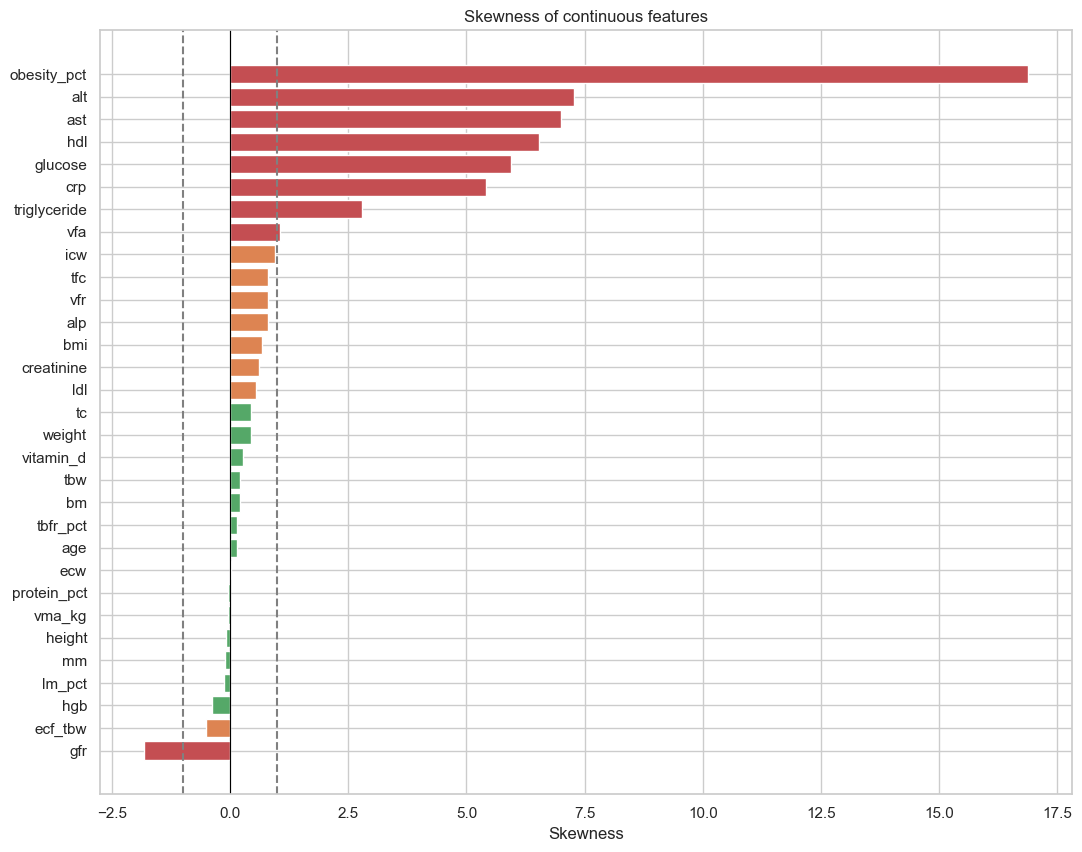
\includegraphics[
        width=0.88\linewidth,
        keepaspectratio
    ]{media/skewness_continous_features.png}
    \caption{Skewness of the continuous variables. The dashed vertical lines
    indicate the threshold of $|\mathrm{skewness}| = 1$ used to identify
    strongly skewed variables.}
    \label{fig:continuous-skewness}
\end{figure}

Figure~\ref{fig:continuous-skewness} shows that several continuous measurements
were strongly right-skewed. The most extreme case was
\texttt{obesity\_pct}, with a skewness of approximately 16.87, followed by
ALT (7.28), AST (6.99), HDL (6.53), glucose (5.94), and CRP (5.41).
Triglyceride was also strongly positively skewed (2.79), while GFR exhibited
substantial negative skewness ($-1.81$). VFA showed a smaller but still notable
positive skewness of approximately 1.06. In contrast, most of the remaining
continuous measurements were relatively close to symmetric.

These results are consistent with the earlier outlier analysis. In particular,
the extreme skewness of \texttt{obesity\_pct} appears to be strongly influenced
by the unusually large observation identified during data-quality assessment.
Similarly, the long right tails observed for ALT, AST, glucose, CRP, and
triglyceride indicate that a small number of participants have measurements
considerably larger than the majority of the sample. These observations were
not removed solely because they increased skewness, since extreme values may
represent clinically plausible measurements.


\subsection{Data Construction}
\label{subsec:data-construction}

The data-construction stage focused on producing a consistent analytical dataset
while preserving the original source data. No additional derived clinical
variables were introduced unless they had a clear analytical justification.

Three logical versions of the dataset were maintained:

\begin{itemize}
    \item \textbf{Raw data:} the original dataset retained without
          modification;

    \item \textbf{Cleaned data:} the dataset after validation of field names,
          data types, categorical values, ranges, duplicates, and potential
          data-quality issues;

    \item \textbf{Model-ready data:} the final analytical dataset containing
          \textit{Gallstone Status} and the predictor variables used by the
          Python modelling pipeline.
\end{itemize}

This separation ensures that preprocessing operations do not overwrite the
source dataset and allows each transformation to be reproduced from the raw
data through the Python scripts.


\subsubsection{Data Partitioning}
\label{subsubsec:data-partitioning}
Before feature selection and model development, two complementary data-splitting
and evaluation strategies were adopted to assess model performance and
robustness: a stratified 70--15--15 holdout split and a
\textit{Leave-One-Patient-Out} (LOPO) cross-validation procedure.

\paragraph{Strategy 1: Stratified 70--15--15 Holdout Split}

For the primary holdout evaluation, the model-ready dataset was partitioned
using the \texttt{scikit-learn} library with stratification based on
\textit{Gallstone Status}. The following proportions were used:

\begin{itemize}

    \item \textbf{70\% Training set:} used for preprocessing decisions,
          feature selection, and model fitting;

    \item \textbf{15\% Validation set:} used for model comparison,
          hyperparameter tuning, threshold analysis, and model-selection
          decisions;

    \item \textbf{15\% Test set:} retained for the final evaluation of the
          selected modelling approach on previously unseen observations.

\end{itemize}

Stratification was used to preserve the approximately balanced distribution of
participants with and without gallstones across the three subsets. This was
particularly important given the relatively small dataset because substantial
differences in class proportions between partitions could otherwise introduce
additional variability into the evaluation results.

The partitioning process can be represented conceptually as follows:

\begin{figure}[H]
    \centering

    \fbox{
        \parbox{0.90\linewidth}{
            \centering

            \textbf{Model-ready Dataset}

            \vspace{0.3cm}

            $\downarrow$

            \vspace{0.3cm}

            \textbf{Stratified Partition by Gallstone Status}

            \vspace{0.4cm}

            \begin{tabular}{ccc}
                \textbf{70\% Training}
                &
                \textbf{15\% Validation}
                &
                \textbf{15\% Test}
                \\[0.2cm]

                Feature selection
                &
                Model comparison
                &
                Final evaluation
                \\

                Model fitting
                &
                Parameter tuning
                &
                Unseen observations
            \end{tabular}
        }
    }

    \caption{Training, validation, and testing strategy used in the Python
    modelling workflow.}
    \label{fig:partition-workflow}
\end{figure}

Feature-selection decisions and model fitting were performed using only the
training partition. The validation partition was subsequently used to compare
candidate models and tune modelling choices. The final test partition remained
separate from these stages and was used only after the modelling strategy had
been established.

\paragraph{Strategy 2: Leave-One-Patient-Out Evaluation}

A second evaluation strategy, referred to as
\textit{Leave-One-Patient-Out} (LOPO), was used to provide an additional
assessment of model robustness on unseen patients. LOPO corresponds to
leave-one-out cross-validation at the patient level. During each iteration, one
patient was held out for evaluation while all remaining patients were used for
model training.

For a dataset containing $N$ patients, the procedure generates $N$ model-fitting
iterations:

\[
\mathcal{D}_{\mathrm{train}}^{(i)}
=
\mathcal{D} \setminus \{P_i\},
\qquad
\mathcal{D}_{\mathrm{test}}^{(i)}
=
\{P_i\},
\]

where $P_i$ denotes the patient excluded from the training data during
iteration $i$.

This process was repeated until every patient had served once as the unseen
evaluation case. The predictions generated across all iterations were then
combined to calculate the overall evaluation metrics.

The LOPO strategy differs from the holdout approach because almost the entire
dataset is available for model fitting during each iteration. This is
particularly useful for the Gallstone dataset because of its relatively small
sample size and provides an assessment of whether the model can generalise to
an individual patient who was completely excluded from the corresponding
training process.

The two strategies were evaluated separately. The 70--15--15 split provides a
conventional development framework with independent training, validation, and
test partitions, while LOPO evaluates model stability and patient-level
generalisation across the complete dataset. Using both approaches provides a
more comprehensive assessment of predictive performance than relying on a
single data split alone.

These separation reduces the risk of information leakage and provides a more
independent estimate of how well the resulting model is expected to generalise
to previously unseen patient observations.

Any preprocessing operation that required parameters to be estimated from the
data was fitted using the training partition only and subsequently applied to
the validation and test partitions. This principle applies, for example, to
feature scaling, statistical transformations, and model-based feature
selection.


\subsection{Data Integration}
\label{subsec:data-integration}

Although the Gallstone dataset was originally obtained as a single public
dataset, an explicit integration exercise was conducted to demonstrate how
logically separate healthcare data sources can be combined into a unified
analytical table.

The original dataset was preserved unchanged and divided into two logical CSV
sources. The first file,
\texttt{gallstone\_demographic\_clinical.csv}, contains 319 records and
9 fields describing demographic and clinical characteristics. The second file,
\texttt{gallstone\_biological\_body\_composition.csv}, contains the same
319 participants and 33 fields describing biological, laboratory, and
body-composition measurements.

A unique \texttt{record\_id}, ranging from 1 to 319, was included in both
tables as the one-to-one integration key. Both tables also contained
\textit{Gallstone Status} so that target consistency could be verified before
integration. However, \textit{Gallstone Status} was not used as a merge key
because it does not uniquely identify an individual participant.

Integration was implemented using the \texttt{pandas.merge()} operation with
\texttt{record\_id} as the matching field. The merge was configured as a
one-to-one operation so that duplicate identifiers or unexpected many-to-one
relationships could be detected explicitly.

Post-integration quality checks verified that all 319 participant records were
retained and that no unmatched identifiers or additional missing values were
introduced by the merge.

The duplicated \textit{Gallstone Status} fields from the two logical data
sources were compared before one copy was removed from the final analytical
table. The \texttt{record\_id} field was retained for traceability and quality
control but excluded from the predictor set used for model development.

This integration exercise represents a simplified version of a realistic
healthcare environment in which demographic and clinical data may be stored
separately from laboratory or body-composition measurements. The Python
workflow demonstrates how these sources can be integrated while maintaining
record integrity and preventing inappropriate use of the target variable as an
integration key.


\subsection{Data Reformatting}
\label{subsec:data-reformatting}

The original Gallstone dataset was provided in Microsoft Excel format
(\texttt{.xlsx}). The file was loaded programmatically using
\texttt{pandas.read\_excel()} and subsequently exported to comma-separated
values (\texttt{.csv}) where appropriate for intermediate storage and
reproducible processing.

CSV was selected as an intermediate format because it provides a simple,
platform-independent representation of tabular data and avoids spreadsheet
formatting that is irrelevant to the modelling process. The use of CSV was not
a modelling requirement, however, because the Python pipeline can also operate
directly on Excel or other structured tabular formats.

During reformatting, variable names were standardised and unnecessary
spreadsheet-specific formatting was removed. The resulting fields were then
classified according to their analytical meaning.

Continuous clinical and body-composition measurements, such as BMI, glucose,
triglyceride, weight, and total body water, were represented as numerical
variables.

Binary variables such as Coronary Artery Disease, Hypothyroidism,
Hyperlipidemia, and Diabetes Mellitus were stored as categorical or binary
indicators rather than being interpreted as continuous measurements.

Variables representing ordered clinical levels were treated as ordinal
variables when their coding reflected an increasing degree of severity or
disease burden.

The target variable, \textit{Gallstone Status}, was represented internally as a
binary label for model training while human-readable labels
(\textit{Gallstone Absent} and \textit{Gallstone Present}) were used in
tables and visualisations.

The final model-ready dataset therefore contained consistent field names,
validated data types, clearly defined variable roles, and a reproducible schema
that could be used directly by the subsequent Python-based feature engineering
and modelling pipeline.


\subsection{Reproducible Open-Source Preparation Pipeline}
\label{subsec:python-preparation-pipeline}

The complete preparation process was implemented as a script-based
open-source workflow. At a high level, the pipeline consisted of:

\begin{enumerate}
    \item loading the source data using \texttt{pandas};
    \item standardising variable names and data types;
    \item validating missing values, duplicates, coding ranges, and
          observations;
    \item performing exploratory outlier and distribution checks;
    \item integrating logically separated datasets using
          \texttt{pandas.merge()};
    \item constructing the final predictor and target datasets;
    \item creating stratified training, validation, and test partitions using
          \texttt{scikit-learn};
    \item fitting any required preprocessing operations using the training
          subset only; and
    \item passing the resulting datasets to the machine-learning modelling
          pipeline.
\end{enumerate}

The use of an open-source Python stack provides several advantages for this
project. Each operation is explicitly defined in code, preprocessing decisions
can be version-controlled, experiments can be reproduced using fixed random
seeds, and identical transformations can be consistently applied across
multiple candidate models.

The resulting workflow therefore provides a transparent and reproducible
transition from the original Gallstone dataset to the datasets used for model
training, validation, and final evaluation.